% **************************************************************
% Hi! Edit this file for your presentation!
% **************************************************************

% ==================///==================///==================///
% ==================/// LATEX'S STUFF
% ==================///==================///==================///

\documentclass{beamer}
\usepackage{amsfonts,amsmath,oldgerm}
\usepackage{listings}
\usepackage{colortbl}
\usepackage{svg}
\usepackage{listings}
\usetheme{_statale}
\usefonttheme[onlymath]{serif}


\setbeamertemplate{caption}[numbered]
\newcommand{\testcolor}[1]{\colorbox{#1}{\textcolor{#1}{test}}~\texttt{#1}}
\newcommand{\hrefcol}[2]{\textcolor{frmtxt}{\href{#1}{#2}}}
\titlebackground*{assets/background}

% ==================///==================///==================///
% ==================/// SPLASH PAGE
% ==================///==================///==================///

\title{Open Source - An exploration}
\subtitle{Seminar Series Presentation}
\course{Group 18}
%\author{Vincent Boseck{\normalfont , 201610501}\\
%Ignacio Gea Labella{\normalfont , 202303552}\\
%Giacomo Rocca{\normalfont , 202303007}\\
%Colja Stork{\normalfont , 201706290}\\}
\date{March 2024}


% ==================///==================///==================///
% ==================/// START PRESENTATION
% ==================///==================///==================///

\pgfplotsset{compat=1.18}
\usetikzlibrary{positioning}
\begin{document}
\maketitle

% Define the color for all sections in the TOC after the title slide
\setbeamercolor{section in toc title}{fg=toctxt, bg=toctxt}

% Modify the TOC after the title slide to use the new template
\AtBeginSection[]
{
    \begingroup
    \themecolor{main}
    \begin{frame}[allowframebreaks]{Table of Contents}
        \tableofcontents
    \end{frame}
    \endgroup
}


\section{What is Open-Source?}

\begin{frame}[fragile]{Definition of Open Source}
%\addcontentsline{toc}{subsection}{Definition of Open Source}
\makebox[\textwidth][c]{
\begin{figure}
    \centering
    
\includegraphics[width=1.1\linewidth]{assets/Untitled.png}
\end{figure}}
\end{frame}

\automateframe{Key Characteristics}{
\begin{itemize}
    \item Transparency
    \item Collaboration
    \item Community-driven Development
    \item Innovation and Iteration
    \item Freedom to Use and Modify
    \item Licensing
\end{itemize}
}

\begin{frame}[fragile]{Licensing}
\makebox[\textwidth][c]{
\begin{figure}
    \centering
    
\includegraphics[width=1.1\linewidth]{assets/Licenses.png}
\end{figure}
}
\end{frame}



% Define sectioning and table of contents
\AtBeginSection[]
{
    \begingroup
    \themecolor{main}
   \begin{frame}[allowframebreaks]{Table of Contents}
       \tableofcontents[currentsection]
    \end{frame}
   \endgroup
}

\section{Benefits \& Downsides}

\begin{frame}[fragile,allowframebreaks]{Pro\&Con Table}

\begin{table}[]
    \small
    \centering
    \def\arraystretch{1.1}
    \begin{tabular}{|c|c|}
    \hline
      \cellcolor{green!50}\textbf{Pros} & \cellcolor{red!50}\textbf{Cons} \\
    \hline
       $\blacktriangleright$ Transparency & $\blacktriangleright$ Lack of Support \\
       $\blacktriangleright$ Community collaboration & $\blacktriangleright$ Fragmentation \\
       $\blacktriangleright$ Customization & $\blacktriangleright$ Perceived Lack of Accountability \\
       $\blacktriangleright$ Cost-Effective & \\
       $\blacktriangleright$ Innovation and rapid development & \\
       $\blacktriangleright$ Vendor Independence & \\
       $\blacktriangleright$ Learning Opportunities & \\
        $\blacktriangleright$ Ethical Considerations & \\
    \hline
    \end{tabular}
    \caption{Pros and Cons}
    \label{tab:ProsCons}
\end{table}
    
\end{frame}

\section{Case Study}

\begin{frame}[fragile,allowframebreaks]{Open Source Projects}
    
\begin{figure}
    \centering
    
\includegraphics[width=0.42\linewidth]{assets/signal-2024-03-12-131914_002.png}
    % \caption{Open Source Projects}
    % \label{fig:enter-label}
\end{figure}

\end{frame}

\begin{frame}[fragile,allowframebreaks]{Enterprise Resource Planning Systems}
    
\begin{figure}
    \centering
    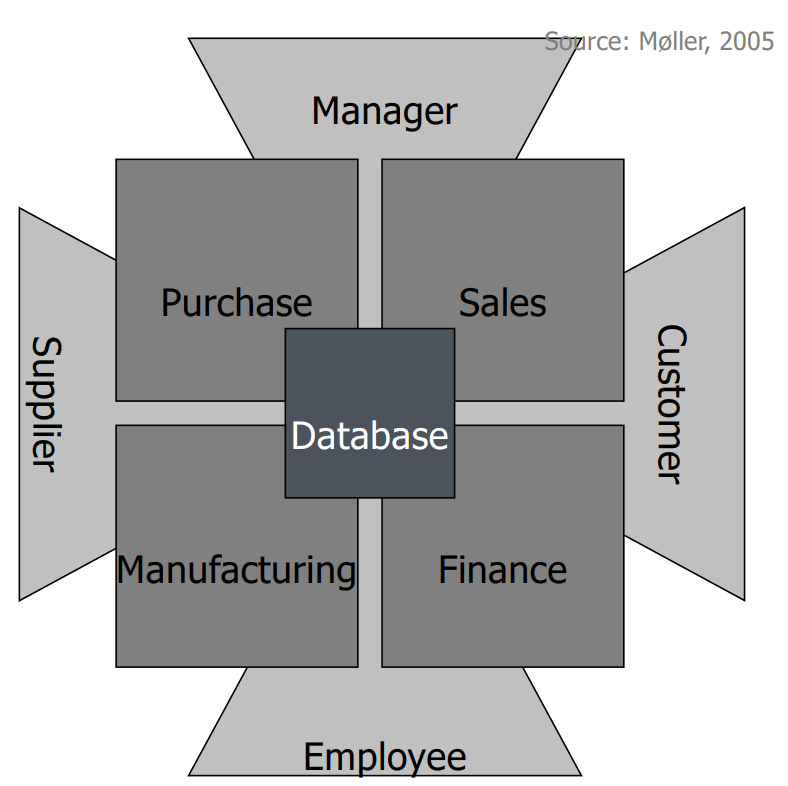
\includegraphics[width=0.40\linewidth]{assets/ERP.png}
    % \caption{Open Source Projects}
    % \label{fig:enter-label}
\end{figure}

\end{frame}

\begin{frame}[fragile,allowframebreaks]{SAP}
    
\begin{figure}
    \centering
    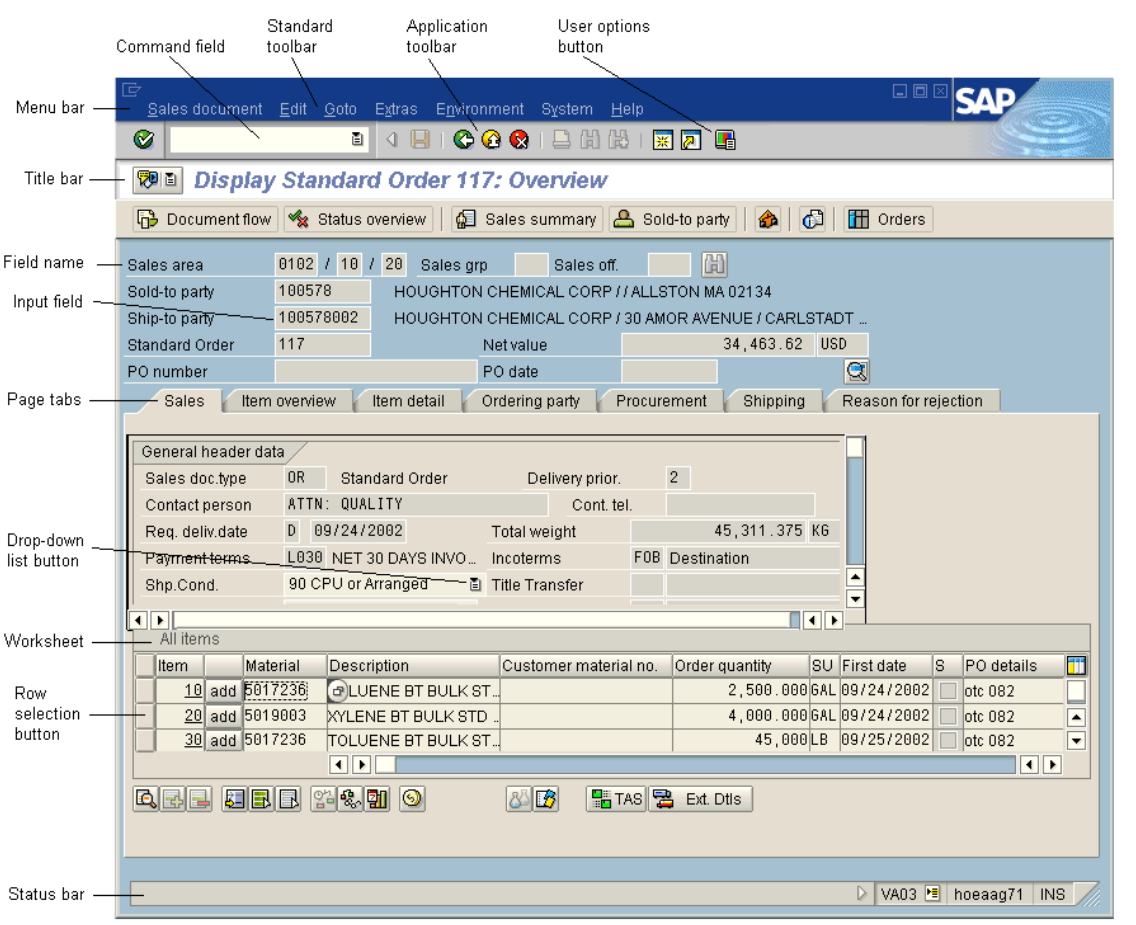
\includegraphics[width=0.50\linewidth]{assets/SAP.png}
    % \caption{Open Source Projects}
    % \label{fig:enter-label}
\end{figure}

\end{frame}
\begin{frame}[fragile,allowframebreaks]{Odoo}
    
\begin{figure}
    \centering
    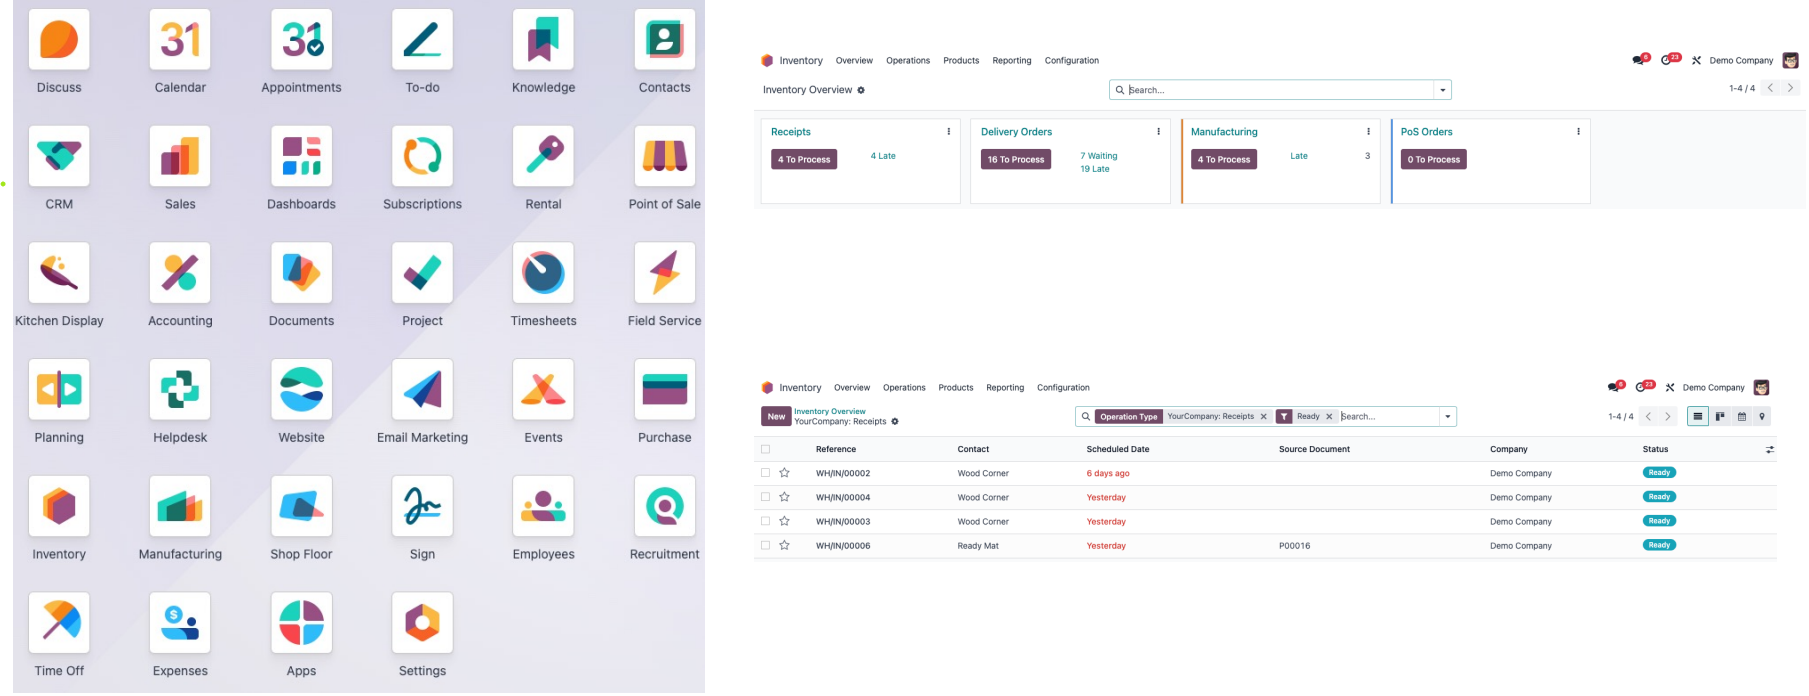
\includegraphics[width=0.90\linewidth]{assets/OdooInterface.png}
    % \caption{Open Source Projects}
    % \label{fig:enter-label}
\end{figure}

\end{frame}

\begin{frame}[fragile,allowframebreaks]{Odoo Key Characteristics}
\begin{itemize}
    \item Transparency
    \item Collaboration
    \item Community-driven Development
    \item Transparency
    \item Freedom to Use and Modify
    \item Licensing
\end{itemize}
    
\end{frame}

\begin{frame}[fragile,allowframebreaks]{Price Comparison}
    
\begin{figure}
    \centering
    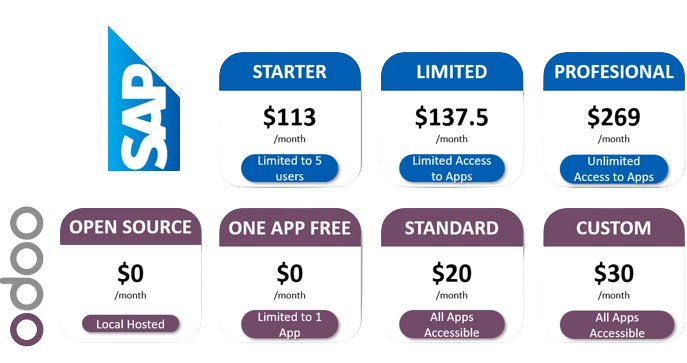
\includegraphics[width=0.70\linewidth]{assets/OdooPrices-removebg-preview.png}
    % \caption{Open Source Projects}
    % \label{fig:enter-label}
\end{figure}
\end{frame}

\begin{frame}[fragile,allowframebreaks]{What is TensorFlow?}
    \begin{columns}[T]
        \column{0.99\textwidth}
            \vspace{1cm}
            \begin{itemize}
                \item Platform for machine learning
                \begin{itemize}
                    \item Machine learning library
                \end{itemize}
                \item Free and open source
                \begin{itemize}
                    \item License: Apache license 2.0
                    \item Initially from Google
                \end{itemize}
            \end{itemize}
        
         \column{0.01\textwidth}
             \vspace{-1cm}
             \hspace*{-4cm}
             
\includegraphics[width=4cm]{assets/TensorFlow_logo_tp.png}
    \end{columns}
\end{frame}

\begin{frame}[fragile,allowframebreaks]{What is TensorFlow?}
    \begin{columns}[T]
        \column{0.99\textwidth}
            \vspace{1cm}
                \begin{itemize}
                    \item Data flow graphs
                    \begin{itemize}
                        \item ML algorithms as a graph of connected operations
                        \item Quick and intuitive work flow
                    \end{itemize}
                \item Works with Python, C++ etc.
                \end{itemize}
         \column{0.01\textwidth}
            \vspace{.5cm}
            \hspace*{-4cm}
            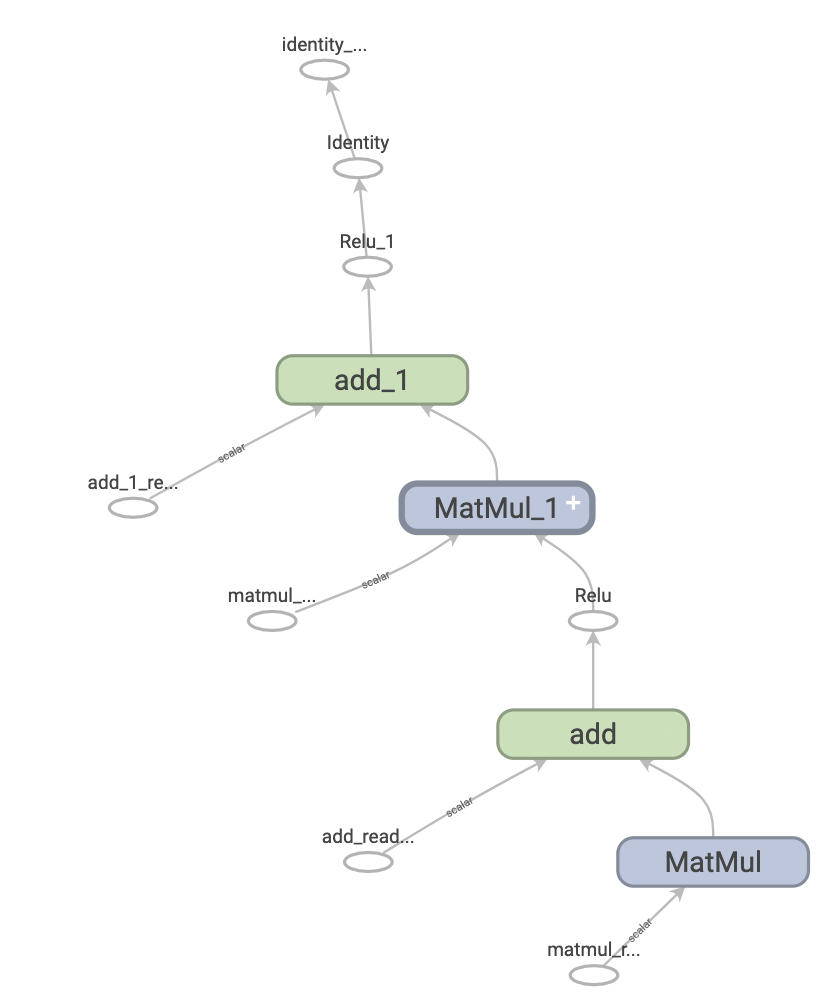
\includegraphics[width=4cm]{assets/TensorFlow_Graph_Example.png} 
                \\
                \vspace{-.1cm}
                \hspace*{-4cm}\caption{Source: tensorflow.org}
    \end{columns}
\end{frame}

\begin{frame}[fragile,allowframebreaks]{What is TensorFlow?}

        \begin{columns}[T]
        \column{0.99\textwidth}
            \vspace{1cm}
            \begin{itemize}
                \item Visualization of work by TensorBoard
                \item Natural language processing
                \item Image recognition
                \item Computational-based simulations
                \item Training and execution on GPU, CPU or TPU (Cloud)
            \end{itemize}
        
         \column{0.01\textwidth}
             \vspace{-0cm}
             \hspace*{-5cm}
             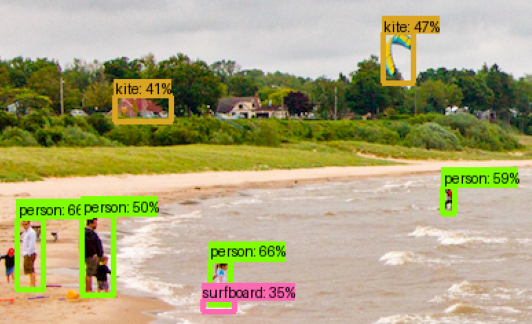
\includegraphics[width=5cm]{assets/TensorFlow_ObjectDetection(2).png}
                 \\
                 \vspace{-.1cm}
                 \hspace*{-5cm}\caption{Source: tensorflow.org}
        \end{columns}
\end{frame}

\begin{frame}[fragile,allowframebreaks]{Tensor flow: Open-source characteristics}
    \begin{itemize}
        \item Google as contributor and promoter
        \item Network of collaborators 
        \item Part of Googles business model
        \item Beyond source code: Sharing of models and datasets
        \item Customization and own ??APIs??
    \end{itemize}
\end{frame}

\begin{frame}[fragile,allowframebreaks]{Tensor flow: Google's perspective}
    \begin{itemize}
        \item Googles AI products use TensorFlow
        \item (Worldwide) collaboration
        \item Shared Datasets and ML models
        \item Googles cloud-TPUs
    \end{itemize}
\end{frame}

\begin{frame}[fragile,allowframebreaks]{Tensor flow: Pros and cons}
    \begin{itemize}
        \item Well-documented
        \item Widely used
        \item Shared Datasets and ML models
        \item Freedom to use and modify
        \item Integration in business model
        \item ???Cons???
    \end{itemize}
\end{frame}

\section{How can I contribute to a project?}

\begin{frame}[fragile,allowframebreaks]{Short answer}

    \begin{figure}
    \centering
    \subfigure{
\includegraphics[width=0.24\textwidth]{assets/GitHub_Logo.png}}\hspace{0.02\textwidth}
    \subfigure{
\includegraphics[width=0.24\textwidth]{assets/Git-Logo-1788C.png}}\hspace{0.02\textwidth}
    \subfigure{
\includegraphics[width=0.26\textwidth]{assets/gitlab-logo-200.png}}
    
    \label{fig:SftwToContribute}
    \end{figure}

\end{frame}

\automateframe{A quick example}{
\begin{itemize}[<+->]
    \item Suppose you want to \textbf{contribute} to a project which is currently working fine
    \item And you want to make a change \textbf{without breaking anything}...
\end{itemize}
}

\begin{frame}{A quick example}
\begin{itemize}
    \item You could use some Cloud Based service and copy your folder and files
\end{itemize}

\begin{figure}
    \centering
    
\includegraphics[width=0.35\linewidth]{assets/dir_chaos.png}
    \label{fig:dir_chaos}
\end{figure}

\end{frame}



\begin{frame}{A quick example}
\begin{itemize}
    \item And find yourself with a real mess...
\end{itemize}

\begin{figure}
    \centering
    
\includegraphics[width=0.35\linewidth]{assets/pure_chaos_nobg.png}
    \label{fig:pure_chaos}
\end{figure}

\end{frame}

\begin{frame}{What is git?}
\begin{itemize}
    \item \textbf{Version Control Software} - such as \href{https://help.autodesk.com/view/VAULT/2023/ENU/?guid=GUID-87D9CA09-9881-4506-9465-0677392BCD7E}{Autodesk Vault}
    \end{itemize}
    
\end{frame}

\begin{frame}{What is git?}
How can I actually use it?

\begin{figure}[htbp]
  \begin{minipage}[t]{0.5\textwidth}
    \begin{block}{Code for a Page with an Itemised List}<+->
    \begin{verbatim}
    \begin{frame}{Writing a Simple Slide}
    \framesubtitle{It's really easy!}
        \begin{itemize}[<+->]
            \item A typical slide has bulleted lists
        \item These can be uncovered in sequence
    \end{itemize}\end{frame}
    \end{verbatim}
\end{block}
  \end{minipage}
  \hfill
  \begin{minipage}[t]{0.4\textwidth}
    \centering
    
\includegraphics[width=\linewidth]{assets/gitlab-logo-200.png}
    \caption{Example Image}
    \label{fig:example}
  \end{minipage}
\end{figure}

\vspace{30pt}
Let's give a look to something more practical now...
    
\end{frame}

\automateframe{A practical guide}{
\begin{enumerate}
    \item \href{https://github.com/}{Create a GitHub Account}
    \item 
    \href{https://github.com/firstcontributions/first-contributions}{Search for the first-contributions project}
    \begin{figure}
        \centering
        
\includegraphics[width=0.75\linewidth]{assets/Screenshot_project.png}
        
        
    \end{figure}
    
    
\end{enumerate}
}

\begin{frame}{A practical guide}
    What are the first files that you should look for in a project?
    \begin{itemize}
    \item \href{https://github.com/firstcontributions/first-contributions/blob/main/README.md}{\textbf{README.md:}}
        \begin{itemize}
            \item Project landing page.
            \item Goals, purpose, how to start, and additional info.
        \end{itemize}
    \end{itemize}

\end{frame}

\begin{frame}{A practical guide}
    What are the first files that you should look for in a project?
    \begin{itemize}
    \item \href{https://github.com/firstcontributions/first-contributions/blob/main/Contributors.md}{\textbf{contributing.md:}}
        \begin{itemize}
            \item Details contributions sought by maintainers.
            \item Process for submitting changes or getting involved.
        \end{itemize}
    \end{itemize}

\end{frame}

\begin{frame}{A practical guide}
    What are the first files that you should look for in a project?
    \begin{itemize}
        \item \href{https://github.com/firstcontributions/first-contributions/blob/main/CODE_OF_CONDUCT.md}{\textbf{Code of Conduct (CoC):}}
        \begin{itemize}
            \item Guidelines for community interaction.
            \item Lists unacceptable behaviors and reporting mechanisms.
            \item Indicates positive behaviors encouraged by maintainers.
        \end{itemize}
    \end{itemize}

\end{frame}

\begin{frame}{A practical guide}
    What are the first files that you should look for in a project?
    \begin{itemize}
            \item 
            \href{https://github.com/firstcontributions/first-contributions/blob/main/LICENSE}{\textbf{license.txt:}}
        \begin{itemize}
            \item Specifies open source license.
            \item Contains full license text.
            \item Essential for understanding usage, modification, and enhancement permissions.
        \end{itemize}
    \end{itemize}

\end{frame}

\begin{frame}{A practical guide}
    \begin{enumerate}
        \item Done
        \item Done
        \item Follow the step by step guide and start contributing
    \end{enumerate}
\end{frame}


% ==================///==================///==================///
% ==================/// END PRESENTATION
% ==================///==================///==================///

\begin{frame}[c]
\centering
\begin{minipage}{\textwidth}
  \usebeamercolor[fg]{normal text}
  \centering
  \ifstrequal{#1}{notitle}{}{
    \huge \inserttitle
    \vspace{5mm}
  }
  \Large \textsl{\\Thank you}
  \begin{figure}
      \centering
      
\includegraphics[width=0.25\linewidth]{assets/QR-Code.png}
  \end{figure}
\end{minipage}
\end{frame}


%\backmatter
\end{document}